% Provenance (never printed): see sources/outline_sources.md (Year 3: Gibbs
% energy and the phase rule in rocks, chemical potential recalled from the
% chemistry book; ternary diagrams; pseudosections, principle). Brief:
% sources/book5/BRIEFS.md, ch. 11. Curves from figdata/bachelor-3/
% gasp_tables.py, schreinemakers.py and regular_solution.py. Exercise and
% problem values in the Book 5 scratch calculator calc/ch11.py.
\chapter{Termodinámica de las rocas}\label{ch:b3:petrological-thermodynamics}

Un granate de unos pocos milímetros de diámetro creció zona a zona mientras su esquisto se enterraba
y se calentaba. Su borde aún registra, en sus contenidos de calcio, hierro y magnesio, el
último equilibrio que alcanzó con la biotita y el plagioclasa que lo rodean. El
volumen de segundo año convirtió tales composiciones en una temperatura y una presión mediante
dos ecuaciones calibradas. Este capítulo abre esa caja: de dónde proceden las ecuaciones,
y hasta dónde son fiables las tablas de entalpías y entropías medidas,
cuántos minerales puede albergar una roca, cómo se mezclan las soluciones sólidas y
se desmezclan, y cómo un ordenador convierte una composición global en un mapa de las
asociaciones que debe mostrar.

\begin{recall}
La energía de Gibbs, el potencial químico, la actividad y la constante de
equilibrio, la varianza y la regla de las fases, la laguna de miscibilidad y la
regla de la palanca se encuentran en los volúmenes universitarios de los libros de química. La reacción univariante,
su pendiente de Clapeyron $\Delta_rS/\Delta_rV$, el punto invariante y el
diagrama de aluminosilicatos calculado a partir de tablas se encuentra en el volumen de segundo año, en su
capítulo sobre facies metamórficas; el geotermómetro y el geobarómetro, el
termómetro de intercambio granate--biotita y el barómetro GASP, en su capítulo sobre
trayectorias P--T--t; los diagramas ternarios y el cotéctico, en su capítulo sobre magmas. Una
solución sólida y sus miembros extremos se encuentran en el volumen de primer año, en su capítulo sobre
minerales.
\end{recall}

\section{Equilibrio a partir de tablas}\label{sec:b3:petrological-thermodynamics:tables}

Para una reacción entre minerales de composición fija, el equilibrio a la
temperatura $T$ y presión $P$ es $\Delta_rG(T, P) = 0$. Las tablas dan, a
\qty{298.15}{K} y \qty{1}{bar}, la entalpía de formación, la entropía y
el volumen molar de cada mineral y la capacidad calorífica $C_p(T)$ anterior. El
volumen de segundo año tomó $\Delta_rH$, $\Delta_rS$ y $\Delta_rV$ como constantes. El
resultado general es el siguiente.

\begin{theorem}[Energía de Gibbs de una reacción a $T$ y $P$]\label{thm:b3:petrological-thermodynamics:dg}
Sea una reacción que tiene, a $T_0 = \qty{298.15}{K}$ y \qty{1}{bar}, la
entalpía $\Delta_rH^\circ$ y entropía $\Delta_rS^\circ$, la variación de la capacidad calorífica
$\Delta_rC_p(T)$ y, entre los sólidos, una variación de volumen $\Delta_rV$
independiente de $T$ y $P$. Entonces
\[
  \Delta_rG(T, P) = \Delta_rH^\circ + \int_{T_0}^{T}\Delta_rC_p\,\mathrm dT
  - T\Bigl(\Delta_rS^\circ + \int_{T_0}^{T}\frac{\Delta_rC_p}{T}\,\mathrm dT\Bigr)
  + (P - 1)\,\Delta_rV ,
\]
y la línea de equilibrio es $P = 1 - \Delta_rG(T, 1)/\Delta_rV$.
\end{theorem}

\begin{proof}
A \qty{1}{bar}, $(\partial\Delta_rH/\partial T)_P = \Delta_rC_p$ y
$(\partial\Delta_rS/\partial T)_P = \Delta_rC_p/T$; integrando desde $T_0$
se obtienen $\Delta_rH(T)$ y $\Delta_rS(T)$, y $\Delta_rG = \Delta_rH -
T\Delta_rS$. A $T$ fijo, $(\partial\Delta_rG/\partial P)_T = \Delta_rV$,
constante por hipótesis; integrando de 1 a $P$ se añade $(P - 1)\Delta_rV$.
Imponiendo $\Delta_rG(T, P) = 0$ se obtiene la línea.
\end{proof}

Las dos integrales se compensan en parte: su suma es $\int_{T_0}^T\Delta_rC_p(1 -
T/T')\,\mathrm dT'$, en la que el factor $1 - T/T'$ es negativo y pequeño
donde $T'$ está próximo a $T$. Entre los sólidos, $\Delta_rC_p$ es en sí pequeño,
porque la capacidad calorífica de un mineral es casi la suma de las de sus
óxidos. La aproximación de propiedades constantes es, por tanto, buena, y las
tablas indican cuánto. Para la reacción GASP,
\[
  \ce{3 CaAl2Si2O8 <=> Ca3Al2Si3O12 + 2 Al2SiO5 + SiO2},
\]
la tabla resumen da $\Delta_rH^\circ = \qty{-36.3}{kJ}$,
$\Delta_rS^\circ = \qty{-130.7}{J.K^{-1}}$ y $\Delta_rV =
\qty{-6.61}{J.bar^{-1}}$, así que una línea de pendiente \qty{19.8}{bar/K}; las
tablas de alta temperatura, que incluyen las capacidades caloríficas, dan
$\Delta_rG$ a cada \qty{100}{K}, y las dos líneas difieren en menos de
\qty{0.12}{kbar} hasta \qty{1200}{K} (la figura siguiente).
% ledger: rh95:gasp-298, rh95:gasp-ht

Los experimentos no concuerdan igual de bien. Invertida en una prensa de pistón-cilindro a
900 a \qty{1250}{\celsius}, la reacción queda \qty{0.9}{kbar} por encima de lo que predicen
las tablas a \qty{627}{\celsius} y \qty{1.9}{kbar} por encima a
\qty{927}{\celsius}. Con $\Delta_rV = \qty{-6.61}{J.bar^{-1}}$,
\qty{1.9}{kbar} equivale a un error de \qty{12.6}{kJ} en $\Delta_rH$; las
incertidumbres de las cuatro entalpías de formación, \qty{3.2}{kJ} para
grosularia, \qty{2.0}{kJ} para anortita y cianita, \qty{1.0}{kJ} para
cuarzo, se combinan en unos \qty{8}{kJ} en $\Delta_rH$. La calorimetría fija cada
mineral con unos pocos kilojulios; una reacción entre unidades formulares grandes multiplica
estos errores y los divide por una pequeña variación de volumen.
% ledger: rh95:gasp-298, kn88:gasp

\begin{definition}[Base de datos termodinámicos internamente coherente]\label{def:b3:petrological-thermodynamics:dataset}
Una \emph{base de datos termodinámicos internamente coherente}\index{base de datos termodinámicos internamente coherente}
es una tabla de las propiedades estándar de
numerosos minerales y fluidos (entalpía de formación, entropía, volumen, capacidad calorífica,
dilatación térmica y compresibilidad) ajustadas conjuntamente, dentro de las
incertidumbres de la calorimetría, de modo que todo equilibrio calculado a partir de ella
reproduce los experimentos invertidos con los que se ajustó.
\end{definition}

Una base de datos así se ajusta una vez, por mínimos cuadrados ponderados o por programación
lineal sobre todos los intervalos experimentales a la vez, y después se usa en cada
reacción entre sus minerales, incluidas las reacciones nunca estudiadas en el
laboratorio. Sus valores no son mediciones independientes: una entalpía puede
desplazarse un kilojulio para ajustar una reacción en la que participa. Los valores de
bases de datos distintas nunca deben mezclarse.

\begin{omfigure}
\begin{tikzpicture}
\begin{axis}[omrecord, width=0.78\linewidth, height=0.5\linewidth,
  xlabel={temperatura (\unit{\celsius})}, ylabel={presión (\unit{kbar})},
  xmin=400, xmax=1300, ymin=0, ymax=30, legend style={font=\scriptsize,
  at={(0.03,0.97)}, anchor=north west, legend cell align=left}]
% computed in figdata/bachelor-3/gasp_tables.py
\fill[omLithLime!60] (axis cs:900,19) rectangle (axis cs:1250,28);
\addplot[red!70!black, very thick] table[x=tc, y=p_kn88] {figdata/out/bachelor-3-gasp_tables-lines.dat};
\addlegendentry{experimento (miembros extremos)}
\addplot[omDef, thick, densely dashed] table[x=tc, y=p_const] {figdata/out/bachelor-3-gasp_tables-lines.dat};
\addlegendentry{tablas, $\Delta_rH$, $\Delta_rS$ constantes}
\addplot[omDef, only marks, mark=*, mark size=1.8pt] table[x=tc, y=p_table] {figdata/out/bachelor-3-gasp_tables-tables.dat};
\addlegendentry{tablas, con capacidades caloríficas}
\node[font=\scriptsize, align=center] at (axis cs:1075,26.3) {experimentos\\invertidos};
\node[font=\scriptsize] at (axis cs:560,4) {anortita};
\node[font=\scriptsize, align=center] at (axis cs:560,17) {grosularia + cianita\\+ cuarzo};
\end{axis}
\end{tikzpicture}

\par\smallskip{\small La reacción GASP de los miembros extremos, 3 anortita = grosularia +
2 cianita + cuarzo, calculada a partir de las tablas calorimétricas con propiedades
constantes (discontinua) y con las capacidades caloríficas (puntos), y la recta ajustada
a los experimentos invertidos realizados en el rango sombreado (rojo, extrapolado por debajo de
\qty{900}{\celsius}).}\label{fig:b3:petrological-thermodynamics:gasp}
\end{omfigure}
% ledger: rh95:gasp-298, rh95:gasp-ht, kn88:gasp

\section{La regla de las fases en las rocas}\label{sec:b3:petrological-thermodynamics:phase-rule}

La regla de las fases de la química da la varianza $F = c - p + 2$ de un sistema de
$c$ componentes en $p$ fases. Una roca es un sistema así, y sus minerales muestran
qué parte del plano presión--temperatura se equilibró en.

\begin{proposition}[Regla de las fases mineralógica]\label{prop:b3:petrological-thermodynamics:goldschmidt}
Una roca que ha alcanzado el equilibrio a una presión y una temperatura elegidas
libremente dentro de un área del plano presión--temperatura contiene como máximo tantas
fases como componentes tiene: $p \le c$. Esta es la
\emph{regla de las fases mineralógica}\index{regla de las fases mineralógica}.
\end{proposition}

\begin{proof}
La regla de las fases da $F = c - p + 2$ variables intensivas independientes. Si la
presión y la temperatura pueden variar ambas sin cambiar la asociación, dos
de ellas son libres: $F \ge 2$, luego $p \le c$. Una roca con $p = c + 1$ fases se sitúa
sobre una línea univariante; con $p = c + 2$, en un punto invariante; ninguna de las dos
situaciones es probable en una roca tomada al azar.
\end{proof}

Una roca que incumple la regla o bien se equilibró sobre una línea de reacción, lo que sus
texturas pueden mostrar, o bien nunca alcanzó el equilibrio como conjunto: son causas
frecuentes las texturas de corona, los minerales zonados y los granos relictos. Contar los
componentes requiere cuidado. Un componente presente solo en una fase de composición fija, como
el circón, puede descartarse junto con su fase; un componente fijado por un reservorio externo,
como el agua cuando un fluido atraviesa la roca, no se cuenta como libre, ya que su potencial
químico está impuesto.

Alrededor de un punto invariante, las líneas univariantes no se cortan al azar. En un
sistema de $c$ componentes, $c + 2$ fases se encuentran en el punto y $c + 2$
reacciones irradian de él, cada una escrita entre $c + 1$ fases y nombrada según la
fase que omite, entre corchetes.

\begin{definition}[Análisis de Schreinemakers]\label{def:b3:petrological-thermodynamics:schreinemakers}
El \emph{análisis de Schreinemakers}\index{analisis de Schreinemakers@análisis de Schreinemakers} es el método
que ordena las líneas univariantes alrededor de un punto invariante a partir de las
composiciones de las fases por sí solas, antes de cualquier medida de sus
propiedades termodinámicas: fija el orden de las líneas, el lado de cada
línea que es estable y las asociaciones de cada sector comprendido entre ellas.
\end{definition}

\begin{method}[Reglas de Schreinemakers]\label{met:b3:petrological-thermodynamics:schreinemakers}
(1) Escríbanse las $c + 2$ reacciones, cada una sin una fase. (2) Cada línea es
estable a un lado del punto y metaestable al otro. (3) La prolongación
metaestable de la línea ($i$), que omite la fase $i$, se sitúa en
un sector donde $i$ es estable. (4) Ningún sector comprendido entre dos líneas estables consecutivas
abarca más de \ang{180}. (5) A través de una línea, las asociaciones a ambos lados
son las de los dos lados de su reacción. Fijar una línea con datos entonces
fija todo el haz, salvo una imagen especular.
\end{method}

El punto triple aluminosilicático del volumen de segundo año es el caso más sencillo,
$c = 1$ y tres líneas. La figura siguiente muestra un caso de dos componentes
calculado minimizando la energía de Gibbs en cada punto.

\begin{omfigure}
\begin{tikzpicture}
\begin{axis}[omrecord, width=0.62\linewidth, height=0.5\linewidth,
  xlabel={temperatura (\unit{\celsius})}, ylabel={presión (\unit{kbar})},
  xmin=400, xmax=800, ymin=1, ymax=9, grid=none]
% computed in figdata/bachelor-3/schreinemakers.py
\addplot[omDef, very thick] table[x=t, y=p] {figdata/out/bachelor-3-schreinemakers-ray_A_s.dat};
\addplot[omDef, thick, densely dashed] table[x=t, y=p] {figdata/out/bachelor-3-schreinemakers-ray_A_m.dat};
\addplot[omDef, very thick] table[x=t, y=p] {figdata/out/bachelor-3-schreinemakers-ray_B_s.dat};
\addplot[omDef, thick, densely dashed] table[x=t, y=p] {figdata/out/bachelor-3-schreinemakers-ray_B_m.dat};
\addplot[omDef, very thick] table[x=t, y=p] {figdata/out/bachelor-3-schreinemakers-ray_C_s.dat};
\addplot[omDef, thick, densely dashed] table[x=t, y=p] {figdata/out/bachelor-3-schreinemakers-ray_C_m.dat};
\addplot[omDef, very thick] table[x=t, y=p] {figdata/out/bachelor-3-schreinemakers-ray_D_s.dat};
\addplot[omDef, thick, densely dashed] table[x=t, y=p] {figdata/out/bachelor-3-schreinemakers-ray_D_m.dat};
\node[font=\scriptsize, fill=white, inner sep=1pt] at (axis cs:740,7.85) {(A)};
\node[font=\scriptsize, fill=white, inner sep=1pt] at (axis cs:540,8.75) {(C)};
\node[font=\scriptsize, fill=white, inner sep=1pt] at (axis cs:540,1.6) {(B)};
\node[font=\scriptsize, fill=white, inner sep=1pt] at (axis cs:740,2.15) {(D)};
\node[font=\scriptsize, align=center] at (axis cs:592,7.7) {A + B\\B + D};
\node[font=\scriptsize, align=center] at (axis cs:450,5.0) {A + D};
\node[font=\scriptsize, align=center] at (axis cs:592,2.4) {A + C\\C + D};
\node[font=\scriptsize, align=center] at (axis cs:765,5.0) {A + B\\B + C\\C + D};
\end{axis}
\end{tikzpicture}

\par\smallskip{\small Un haz de Schreinemakers en un sistema de dos componentes con
cuatro fases de composiciones A (0), B ($1/3$), C ($2/3$) y D (1),
calculado para propiedades inventadas: líneas estables sólidas, prolongaciones metaestables
discontinuas, y los pares estables en cada sector. (D) es A + C = 2B, (A) es B + D =
2C, (C) es 2A + D = 3B y (B) es A + 2D = 3C.}\label{fig:b3:petrological-thermodynamics:schreinemakers}
\end{omfigure}

\section{Soluciones sólidas}\label{sec:b3:petrological-thermodynamics:solutions}

La mayoría de los minerales formadores de rocas son soluciones sólidas, y sus miembros extremos aparecen
en las reacciones a través de sus actividades. El volumen de segundo año tomó $a = X^3$ para
la grosularia de un granate y $a = X$ para la anortita de una plagioclasa.
Ambos son casos de un mismo modelo.

\begin{definition}[Modelo de actividad de mezcla en sitios]\label{def:b3:petrological-thermodynamics:site-mixing}
En un \emph{modelo de actividad de mezcla en sitios}\index{modelo de actividad de mezcla en sitios}, los
iones de un mineral se mezclan al azar en cada sitio cristalográfico, de forma independiente
de los demás sitios. La actividad ideal de un miembro extremo es entonces el producto,
sobre los sitios, de la fracción de cada sitio que ocupa elevada al número de
tales sitios por unidad de fórmula: $a_i = \prod_s X_{s,i}^{\,n_s}$.
\end{definition}

Un granate $X_3Y_2\ce{Si3O12}$ tiene tres sitios dodecaédricos $X$ para
\ce{Ca}, \ce{Fe}, \ce{Mg} y \ce{Mn}: $a_{\text{grosularia}} =
X_{\text{Ca}}^3$. Un granate con $X_{\text{Ca}} = 0.10$ contiene
\qty{10}{\percent} de grosularia, pero su actividad es $10^{-3}$. El
modelo ideal cuenta las configuraciones; las soluciones reales tienen además una energía de exceso,
porque iones de tamaños distintos deforman la red.

\begin{definition}[Diagrama energía de Gibbs--composición]\label{def:b3:petrological-thermodynamics:gx}
Un \emph{diagrama energía de Gibbs--composición}\index{diagrama energía de Gibbs--composición}
representa, a temperatura y presión fijas, la energía de Gibbs molar de
cada fase de un sistema frente a su composición. El conjunto estable de cualquier
composición global se sitúa sobre la envolvente convexa inferior de las curvas: una única fase
cuando su curva está en la envolvente, y dos fases en los extremos de una tangente común.
\end{definition}

\begin{proposition}[Solución regular]\label{prop:b3:petrological-thermodynamics:regular}
En una solución binaria con un sitio de mezcla por unidad de fórmula y
energía de interacción $W$, la energía de Gibbs de mezcla es
\[
  G_{\text{mez}} = RT\bigl[x\ln x + (1 - x)\ln(1 - x)\bigr] + Wx(1 - x).
\]
Si $W > 0$, la solución es estable en toda composición por encima de $T_c =
W/(2R)$; por debajo de $T_c$ la curva tiene dos inflexiones y las composiciones
comprendidas entre los dos puntos de su tangente común se separan en dos fases.
\end{proposition}

\begin{proof}
El primer término es $-T$ por la entropía configuracional de la mezcla al azar;
el segundo, la energía de exceso más sencilla, simétrica y nula en ambos extremos.
Derivando dos veces, $G''_{\text{mez}} = RT/[x(1 - x)] - 2W$. Su mínimo
en $x$ está en $x = 1/2$, donde vale $4RT - 2W$, que es positivo para
todo $x$ si $T > W/(2R)$. Por debajo, $G''_{\text{mez}} < 0$ en un intervalo
alrededor de $1/2$: la curva se curva hacia abajo allí, una recta entre dos puntos
de la curva queda por debajo de ella, y según la definición anterior la roca consta de
dos fases.
\end{proof}

\begin{definition}[Solvus, exsolución]\label{def:b3:petrological-thermodynamics:solvus}
El \emph{solvus}\index{solvus} es la curva, en el plano temperatura--composición,
que delimita el intervalo de miscibilidad de una solución sólida: por debajo de ella, un
cristal único de composición intermedia es inestable y se separa en dos.
La \emph{exsolución (mineral)}\index{exsolución (mineral)} es esa separación
dentro de un cristal al enfriarse: láminas de una composición crecen en una matriz de la
otra.
\end{definition}

Los feldespatos alcalinos, los piroxenos y los anfíboles presentan láminas de exsolución,
visibles al microscopio o a simple vista: la pertita de muchos granitos es
un feldespato alcalino exsuelto, una matriz rica en potasio con láminas ricas en
sodio. Entre el \omterm{def:b3:petrological-thermodynamics:solvus}{solvus} y la espinodal, donde $G''_{\text{mez}} = 0$,
un cristal debe primero nuclear la segunda fase; dentro de la espinodal, cualquier pequeña
fluctuación de composición crece solo por difusión.

\begin{omfigure}
\begin{tikzpicture}
\begin{groupplot}[group style={group size=2 by 1, horizontal sep=1.7cm},
  omrecord, width=0.47\linewidth, height=0.42\linewidth, title style={font=\small},
  legend style={font=\scriptsize, legend cell align=left}]
\nextgroupplot[title={(a) Energía de Gibbs de mezcla}, xlabel={$x$},
  ylabel={$G_{\text{mez}}$ (\unit{kJ.mol^{-1}})}, xmin=0, xmax=1, ymin=-9, ymax=1,
  legend style={at={(0.5,0.03)}, anchor=south}]
% computed in figdata/bachelor-3/regular_solution.py
\addplot[black, thick, densely dotted] table[x=x, y=g1500] {figdata/out/bachelor-3-regular_solution-gx.dat};
\addlegendentry{\qty{1500}{K}}
\addplot[red!70!black, thick, densely dashed] table[x=x, y=g1203] {figdata/out/bachelor-3-regular_solution-gx.dat};
\addlegendentry{$T_c = \qty{1203}{K}$}
\addplot[omDef, thick] table[x=x, y=g0900] {figdata/out/bachelor-3-regular_solution-gx.dat};
\addlegendentry{\qty{900}{K}}
\addplot[omDef, thin, forget plot] coordinates {(0.111,-0.635) (0.889,-0.635)};
\nextgroupplot[title={(b) solvus y sección a $X_0 = 0.3$}, xlabel={$x$},
  ylabel={temperatura (\unit{K})}, xmin=0, xmax=1, ymin=600, ymax=1300,
  legend style={at={(0.5,0.03)}, anchor=south}]
\addplot[omDef, thick] table[x=x, y=t_bin] {figdata/out/bachelor-3-regular_solution-solvus.dat};
\addlegendentry{solvus}
\addplot[black, thick, densely dotted] table[x=x, y=t_spin] {figdata/out/bachelor-3-regular_solution-solvus.dat};
\addlegendentry{espinodal}
\addplot[red!70!black, thick, forget plot] coordinates {(0.3,600) (0.3,1300)};
\addplot[red!70!black, thick, densely dashed] table[x=x2, y=t] {figdata/out/bachelor-3-regular_solution-section.dat};
\addlegendentry{isopletas en $X_0$}
\addplot[red!70!black, thick, densely dashed, forget plot] table[x=x1, y=t] {figdata/out/bachelor-3-regular_solution-section.dat};
\node[font=\scriptsize] at (axis cs:0.5,1250) {una fase};
\node[font=\scriptsize] at (axis cs:0.5,950) {dos fases};
\end{groupplot}
\end{tikzpicture}

\par\smallskip{\small Una solución regular con $W = \qty{20}{kJ.mol^{-1}}$
(ilustrativa). (a) Energía de Gibbs de mezcla a tres temperaturas; a
\qty{900}{K} la tangente común (línea fina) toca la curva en $x = 0.11$
y 0.89. (b) El \omterm{def:b3:petrological-thermodynamics:solvus}{solvus} y la espinodal; una roca de composición global $X_0 =
0.3$ (línea vertical roja) es una fase por encima de \qty{1136}{K} y dos
fases por debajo, cuyas composiciones siguen el \omterm{def:b3:petrological-thermodynamics:solvus}{solvus} (discontinua).}\label{fig:b3:petrological-thermodynamics:solvus}
\end{omfigure}

\section{Pseudosecciones}\label{sec:b3:petrological-thermodynamics:pseudosections}

El panel (b) de la figura anterior es ya una pequeña \omterm{def:b3:petrological-thermodynamics:pseudosection}{pseudosección}: para una
composición global, indica qué fases son estables a cada temperatura, y cuáles son sus
composiciones y proporciones. Una roca metamórfica tiene unos diez
componentes y muchas soluciones sólidas, pero el principio es el mismo.

\begin{definition}[Minimización de la energía de Gibbs]\label{def:b3:petrological-thermodynamics:minimisation}
La \emph{minimización de la energía de Gibbs}\index{minimización de la energía de Gibbs} determina, a una
temperatura y presión dadas, el conjunto de fases, sus composiciones y
sus cantidades que minimiza la energía de Gibbs total de un sistema de composición
global fija, sujeta a la conservación de cada componente.
\end{definition}

\begin{definition}[Pseudosección, isopleta, composición global efectiva]\label{def:b3:petrological-thermodynamics:pseudosection}
Una \emph{pseudosección}\index{pseudosección} es un diagrama de fases, normalmente en
el plano presión--temperatura, calculado para una única composición global fija: se
divide en campos, cada uno etiquetado con la asociación que minimiza la
energía de Gibbs allí. Una \emph{isopleta (pseudosección)}\index{isopleta (pseudosección)}
es una línea de una pseudosección a lo largo de la cual una variable composicional
de una fase, o su cantidad, es constante. La \emph{composición global
efectiva}\index{composición global efectiva} es la parte de la composición de la roca
que todavía participa en el equilibrio, una vez eliminados los núcleos de los
cristales zonados, los porfiroblastos aislados de la matriz y otro
material aislado.
\end{definition}

Una \omterm{def:b3:petrological-thermodynamics:pseudosection}{pseudosección} no muestra líneas univariantes en el sentido del
volumen de segundo año: en un sistema con soluciones sólidas, el límite entre dos campos es el
lugar donde una fase aparece o desaparece, y su posición depende de la composición global.
Leerla es directo. La asociación observada fija un campo;
la composición medida de un mineral, el calcio del borde de un granate, por ejemplo,
selecciona una isopleta dentro de él; una segunda isopleta, de otro elemento
u otro mineral, la corta a la presión y temperatura de
equilibrio. Los granates zonados registran una sucesión de cruces de este tipo, uno por cada
zona, a lo largo de la trayectoria de la roca. Pero a medida que el granate crece, su núcleo
retira manganeso y calcio del alcance de la matriz: la \omterm{def:b3:petrological-thermodynamics:pseudosection}{composición global efectiva}
cambia, y la \omterm{def:b3:petrological-thermodynamics:pseudosection}{pseudosección} debe recalcularse para las zonas
posteriores.

\begin{inthelab}[El escritorio del petrólogo]
\begin{minipage}[t]{0.55\linewidth}\vspace{0pt}
El petrólogo estudia primero una lámina delgada al microscopio de polarización,
para identificar la asociación, sus texturas y qué granos crecieron juntos. La misma
lámina, recubierta de carbono, pasa después a una microsonda electrónica, que mide
la composición de puntos de unos pocos micrómetros de diámetro
a lo largo de perfiles a través de los granates. El software que minimiza la energía de Gibbs
con una \omterm{def:b3:petrological-thermodynamics:dataset}{base de datos termodinámicos internamente coherente} y un conjunto de modelos de actividad calcula
una \omterm{def:b3:petrological-thermodynamics:pseudosection}{pseudosección} para la composición global, medida en una lámina de la misma
roca. Sobre ella se representan las isopletas de las composiciones medidas, y allí donde
se cortan está la respuesta. La incertidumbre de la base de datos y de los modelos
de actividad, no la de las medidas, suele ser el factor limitante.
\end{minipage}\hfill
\begin{minipage}[t]{0.42\linewidth}\vspace{0pt}
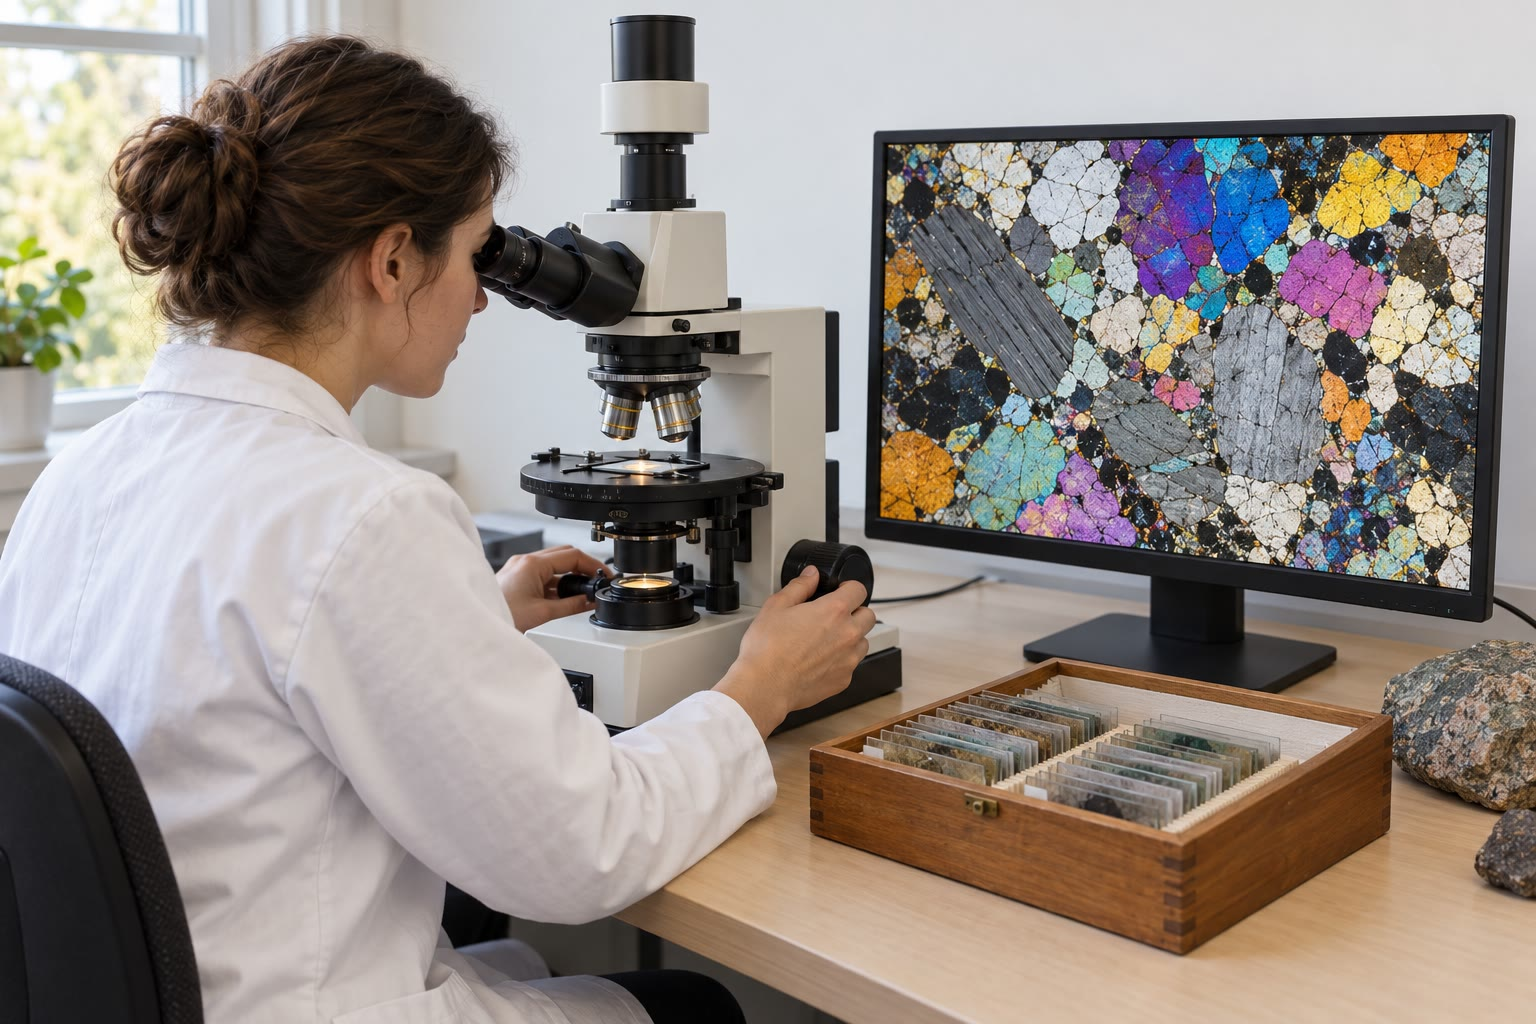
\includegraphics[width=\linewidth]{images/book5/ai/b3-petrology-desk.jpg}

{\scriptsize Un petrólogo ante un microscopio de polarización, con una caja de
láminas delgadas al alcance y una lámina delgada en luz polarizada en la pantalla
(ilustración generada por IA).}
\end{minipage}
\end{inthelab}

\section{Ejercicios}

\begin{exercise}[$\star$]\label{exo:b3:petrological-thermodynamics:1}
A partir de las tablas, la albita tiene $\Delta_fH^\circ = \qty{-3935.0}{kJ}$, $S^\circ =
\qty{207.4}{J.K^{-1}}$, $V = \qty{100.07}{cm^3}$; la jadeíta $-3029.3$, 133.5,
60.40; el cuarzo $-910.7$, 41.5, 22.69 (por mol). Para la reacción albita = jadeíta + cuarzo,
calcúlense $\Delta_rH$, $\Delta_rS$, $\Delta_rV$ (en \unit{J.bar^{-1}}), la
pendiente de Clapeyron y la presión de la línea a \qty{600}{\celsius} con
propiedades constantes.
\end{exercise}
% ledger: rh95:ab-jd-qz

\begin{exercise}[$\star$]\label{exo:b3:petrological-thermodynamics:2}
Una roca del sistema \ce{MgO}--\ce{SiO2} contiene forsterita, enstatita y
cuarzo. Aplíquese la \omterm{prop:b3:petrological-thermodynamics:goldschmidt}{regla de las fases mineralógica}. ¿Qué se concluye?
\end{exercise}

\begin{exercise}[$\star$]\label{exo:b3:petrological-thermodynamics:3}
Calcúlense las actividades ideales de grosularia y piropo en un granate con
$X_{\text{Ca}} = 0.20$ y $X_{\text{Mg}} = 0.15$, y de anortita en una
plagioclasa con $X_{\text{an}} = 0.40$ (un solo sitio).
\end{exercise}

\begin{exercise}[$\star$]\label{exo:b3:petrological-thermodynamics:4}
Calcúlese la temperatura crítica de una solución regular con $W =
\qty{15}{kJ.mol^{-1}}$. ¿Qué $W$ da $T_c = \qty{1000}{K}$?
\end{exercise}

\begin{exercise}[$\star\star$]\label{exo:b3:petrological-thermodynamics:5}
A \qty{1000}{K}, las tablas dan las energías de Gibbs de formación
$-5432.2$ (grosularia), $-3478.1$ (anortita), $-2088.8$ (cianita) y $-730.2$
(cuarzo), en \unit{kJ.mol^{-1}}. Calcúlese $\Delta_rG$ de la reacción GASP a
\qty{1}{bar} y su presión de equilibrio, y compárese con la
línea experimental $P_0 = 22.80\,T - 1093$ (bar, \unit{\celsius}).
\end{exercise}
% ledger: rh95:gasp-ht, kn88:gasp

\begin{exercise}[$\star\star$]\label{exo:b3:petrological-thermodynamics:6}
Para la solución regular de la figura ($W = \qty{20}{kJ.mol^{-1}}$), calcúlese
$G_{\text{mix}}$ en $x = 0.5$ y \qty{900}{K}, y después en el flanco del \omterm{def:b3:petrological-thermodynamics:solvus}{solvus} $x =
0.111$. Demuéstrese que la división de un cristal de composición 0.5 en los dos flancos
disminuye su energía de Gibbs, y en cuánto.
\end{exercise}

\begin{exercise}[$\star\star$]\label{exo:b3:petrological-thermodynamics:7}
¿Cuántas fases concurren en un punto invariante, y cuántas líneas univariantes
parten de él, en un sistema de tres componentes? En el haz de la figura,
compruébese que cada una de las cuatro reacciones está equilibrada.
\end{exercise}

\begin{exercise}[$\star\star$]\label{exo:b3:petrological-thermodynamics:8}
Una roca de composición global $X_0 = 0.3$ en la solución regular de la figura
se ha enfriado a \qty{900}{K}, donde los flancos del \omterm{def:b3:petrological-thermodynamics:solvus}{solvus} son 0.111 y 0.889.
Calcúlese la proporción de cada fase.
\end{exercise}

\begin{exercise}[$\star\star$]\label{exo:b3:petrological-thermodynamics:9}
Con el barómetro GASP $P = P_0 + (3RT/6.21)\ln(X_{\text{Ca}}/X_{\text{an}})$
(bar), calcúlese $\partial P/\partial X_{\text{an}}$ a \qty{900}{K} y
$X_{\text{an}} = 0.30$. ¿En cuánto mueve un error de 0.01 en $X_{\text{an}}$
la presión?
\end{exercise}

\begin{exercise}[$\star\star\star$]\label{exo:b3:petrological-thermodynamics:10}
Demuéstrese que la espinodal de una solución regular es $x(1 - x) = RT/(2W)$. ¿A qué
temperatura un cristal de composición 0.3 se vuelve inestable ante cualquier pequeña
fluctuación, para $W = \qty{20}{kJ.mol^{-1}}$? Compárese con la temperatura a la que
alcanza el \omterm{def:b3:petrological-thermodynamics:solvus}{solvus}, $T = W(1 - 2x)/[R\ln((1 - x)/x)]$, y explíquese la
diferencia.
\end{exercise}

\begin{exercise}[$\star\star\star$]\label{exo:b3:petrological-thermodynamics:11}
Demuéstrese que el \omterm{def:b3:petrological-thermodynamics:solvus}{solvus} de una solución regular simétrica satisface $RT\ln[x/(1 -
x)] + W(1 - 2x) = 0$, y que alcanza su máximo, $T_c = W/(2R)$, en $x
= 1/2$.
\end{exercise}

\begin{exercise}[$\star\star\star$]\label{exo:b3:petrological-thermodynamics:12}
Una roca contiene \qty{2.0}{wt\percent} \ce{MnO}. Los núcleos de granate que contienen
\qty{10}{wt\percent} \ce{MnO} constituyen el \qty{8}{wt\percent} de la roca y están
aislados de la matriz. Calcúlese el contenido de \ce{MnO} de la \omterm{def:b3:petrological-thermodynamics:pseudosection}{composición
global efectiva}. ¿Por qué importa para la \omterm{def:b3:petrological-thermodynamics:pseudosection}{pseudosección} de los bordes del granate?
\end{exercise}

\section{Problema: El granate del esquisto de Varden}

\begin{problem}[{Problema de fin de semana --- la presión y la temperatura de un
esquisto inventado, a partir de tablas, la regla de las fases, modelos de actividad y
termobarometría}]
\label{pb:b3:petrological-thermodynamics:1}
% values: calc/ch11.py; gasp_tables.py
El esquisto del basamento de Varden Hills, metamorfizado hace
\qty{480}{Ma}, contiene granate, biotita, moscovita, plagioclasa, cianita y
cuarzo. En el borde de un granate y en los granos que lo rodean, la microsonda
proporciona: granate $X_{\text{Fe}} = 0.74$, $X_{\text{Mg}} = 0.12$, $X_{\text{Ca}} =
0.10$, $X_{\text{Mn}} = 0.04$; biotita $\ce{Mg}/(\ce{Mg} + \ce{Fe}) = 0.45$;
plagioclasa $X_{\text{an}} = 0.30$. Úsense las tablas de este capítulo para la
reacción GASP, el termómetro del volumen de segundo año
\[
T = \frac{52\,635 + 0.311P}{20.20 - 3R\ln K_D}\quad(T \text{ en K}, P
\text{ en bar}),
\]
y su barómetro experimental $P = 22.80\,t - 1093 + (3RT/6.21)\ln
(X_{\text{Ca}}/X_{\text{an}})$, con $t$ en \unit{\celsius} y $T$ en
kelvin. Tómese $R = \qty{8.314}{J.mol^{-1}.K^{-1}}$, una densidad cortical de
\qty{2800}{kg/m^3} y $g = \qty{9.81}{m/s^2}$.

\medskip\noindent\textbf{Parte I --- Las tablas.}
\begin{enumerate}
  \item A partir de la tabla resumen, calcúlense $\Delta_rH^\circ$, $\Delta_rS^\circ$
        y $\Delta_rV$ de la reacción GASP.
  \item Calcúlese $\Delta_rG$ a \qty{298.15}{K} y \qty{1}{bar}. ¿Qué lado
        es estable en la superficie?
  \item Calcúlese la presión del término extremo a \qty{900}{K} con
        propiedades constantes, y la pendiente de Clapeyron.
  \item Las tablas de alta temperatura dan $\Delta_rG = \qty{81.5}{kJ}$ a
        \qty{900}{K} y \qty{119.8}{kJ} a \qty{1200}{K} (\qty{1}{bar}).
        Calcúlense las presiones.
  \item Compárese con la línea experimental a las mismas temperaturas.
  \item ¿Qué error en $\Delta_rH$ explicaría la discrepancia a \qty{1200}{K}?
        Compárese con la incertidumbre combinada de las cuatro entalpías.
  \item ¿Por qué las capacidades caloríficas cambian tan poco el resultado?
\end{enumerate}

\medskip\noindent\textbf{Parte II --- La regla de las fases.}
\begin{enumerate}[resume]
  \item Enumérense los componentes necesarios para describir los seis minerales y un
        fluido acuoso, y cuéntense las fases.
  \item Calcúlese la variancia con la regla de las fases y compruébese la
        \omterm{prop:b3:petrological-thermodynamics:goldschmidt}{regla de las fases mineralógica}.
  \item Una segunda muestra contiene cianita y silimanita una junto a otra. ¿Qué
        indica sobre su presión y su temperatura?
  \item Durante el metamorfismo circuló agua por la roca. ¿Cómo cambia eso
        el recuento?
\end{enumerate}

\medskip\noindent\textbf{Parte III --- Actividades y termobarometría.}
\begin{enumerate}[resume]
  \item Calcúlense las actividades ideales de grosularia y anortita, y $\ln K$
        de la reacción GASP en la roca.
  \item Calcúlese $K_D$ del intercambio granate--biotita.
  \item Calcúlese la temperatura a \qty{8}{kbar}.
  \item Calcúlese la presión GASP a esa temperatura.
  \item Itérese hasta la intersección de las dos ecuaciones.
  \item Repítase la intersección con la línea del término extremo de las tablas en lugar
        de la línea experimental (con $\Delta_rV = \qty{-6.61}{J.bar^{-1}}$).
        ¿Qué resultado se mantiene y por qué?
  \item ¿Cuánto desplaza el resultado un error de 0.05 en
        $X_{\text{an}}$?
\end{enumerate}

\medskip\noindent\textbf{Parte IV --- El enterramiento.}
\begin{enumerate}[resume]
  \item Con las propiedades constantes del volumen de segundo año, cianita =
        silimanita tiene $\Delta_rH = \qty{7.7}{kJ}$, $\Delta_rS =
        \qty{12.6}{J.K^{-1}}$, $\Delta_rV = \qty{0.571}{J.bar^{-1}}$. ¿Está el
        resultado en el campo de la cianita?
  \item Calcúlese la profundidad de enterramiento.
  \item El núcleo del granate tiene $X_{\text{Ca}} = 0.07$ y creció con plagioclasa
        de igual $X_{\text{an}}$, a una temperatura parecida. ¿Se formó el
        núcleo a mayor o menor profundidad que el borde?
  \item Indíquense la presión máxima y la profundidad de enterramiento del esquisto de Varden.
\end{enumerate}
\end{problem}
